% Section content template for individual Educative lessons
% This file contains the actual content for a specific section
% Generated from Educative API section content

% Section: Introduction to Distributed Logging
% Section ID: 5621964999229440
% Section Slug: introduction-to-distributed-logging
% Generated: 2025-12-07T22:01:03.287837

\subsection{Logging in a distributed system}\label{uWMslz_9KcWXvv0a5y5s1}
\\
In today's world, an increasing number of designs are moving to microservice architecture instead of monolithic architecture. In microservice architecture, logs of each microservice are accumulated in the respective machine. If we want to know about a certain event that was processed by several microservices, it is difficult to go into every node, figure out the flow, and view error messages. But , it becomes handy if we can trace the log for any particular flow from end to end.
\\
Moreover, it is also not necessary that a microservice is deployed on only one node. It can be deployed on thousands of nodes. Consider the following example, where hundreds of microservices are interdependent, and failure of one service can result in failures of other services. And if we do not have logs, we might not determine the root cause of failure. This emphasizes the need for logging.

\begin{figure}[htbp]
 \centering
 \begin{subfigure}[b]{0.48\textwidth}
 \centering
 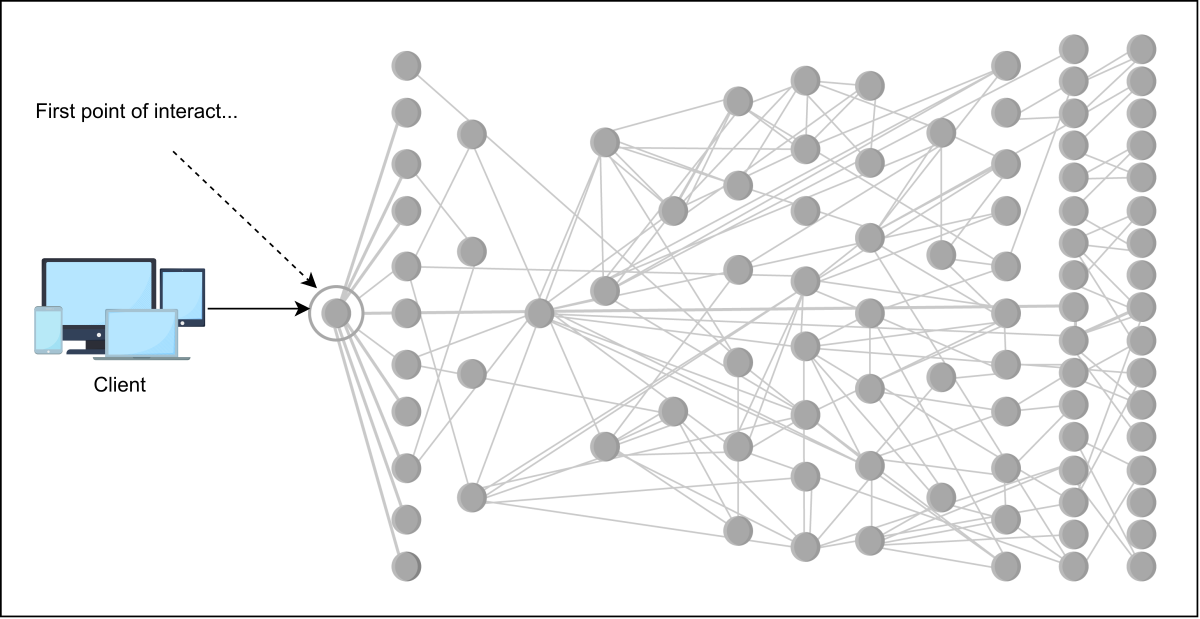
\includegraphics[width=\textwidth]{Images/chapter_22/section_5621964999229440/4571916430868480.png}
 \caption{First point of interaction for client in a distributed systems}
 \end{subfigure}
 \hfill
 \begin{subfigure}[b]{0.48\textwidth}
 \centering
 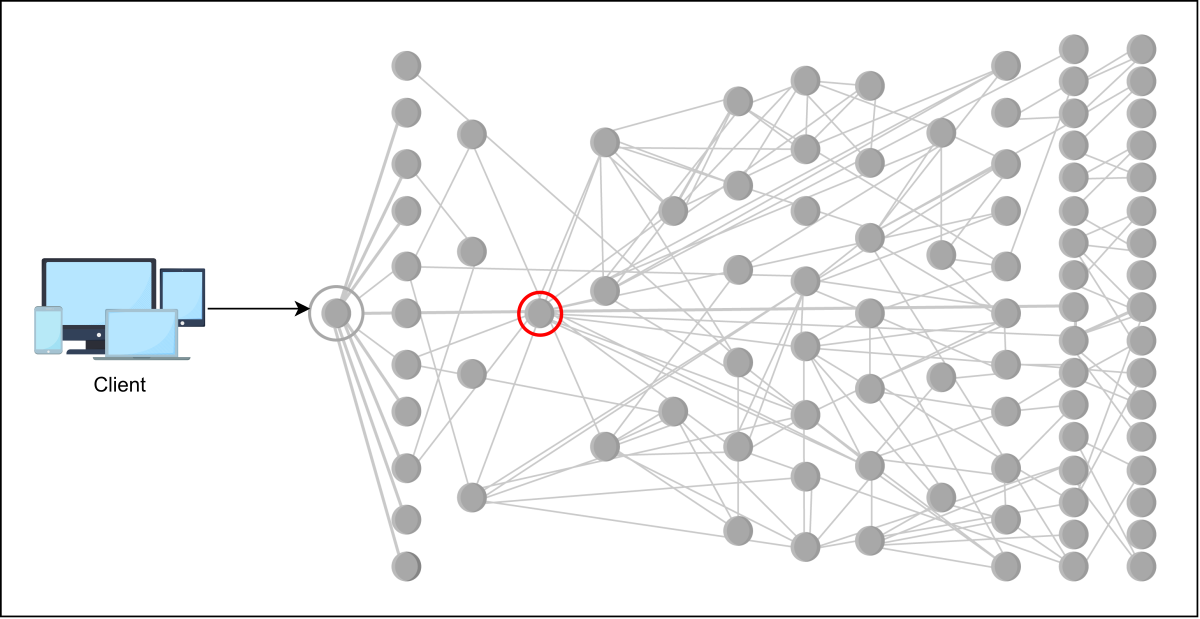
\includegraphics[width=\textwidth]{Images/chapter_22/section_5621964999229440/6733028301602816.png}
 \caption{A service fails in a distributed systems}
 \end{subfigure}
\end{figure}

\begin{figure}[htbp]
 \centering
 \begin{subfigure}[b]{0.48\textwidth}
 \centering
 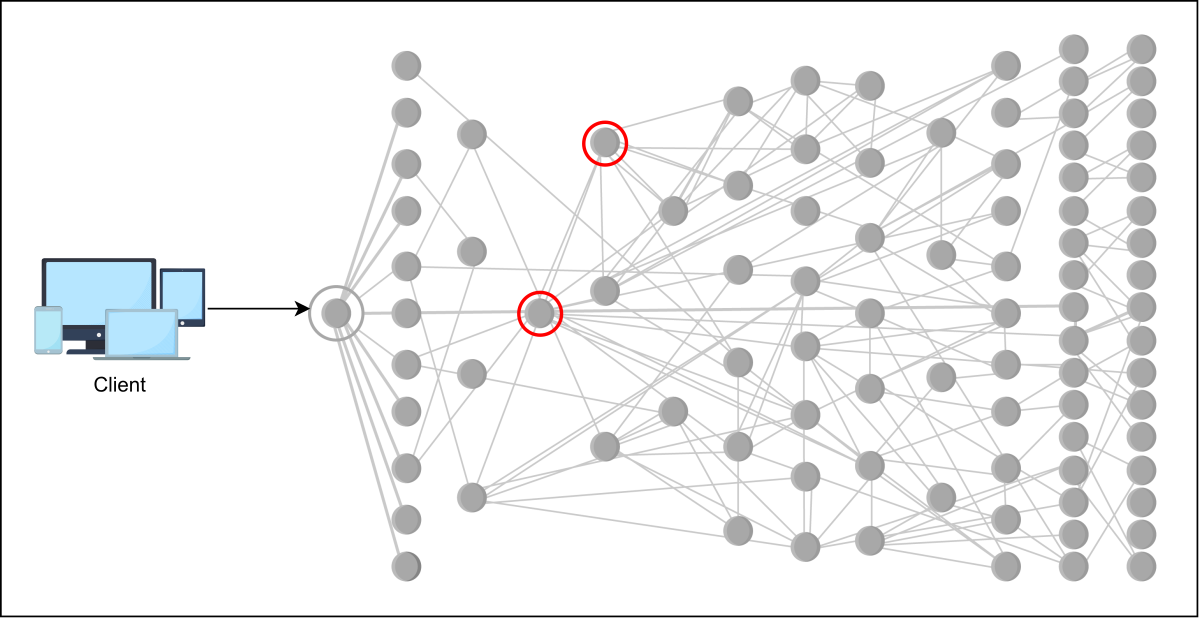
\includegraphics[width=\textwidth]{Images/chapter_22/section_5621964999229440/5313872048029696.png}
 \caption{Another service that was dependent on the previous service also failed because of it}
 \end{subfigure}
 \hfill
 \begin{subfigure}[b]{0.48\textwidth}
 \centering
 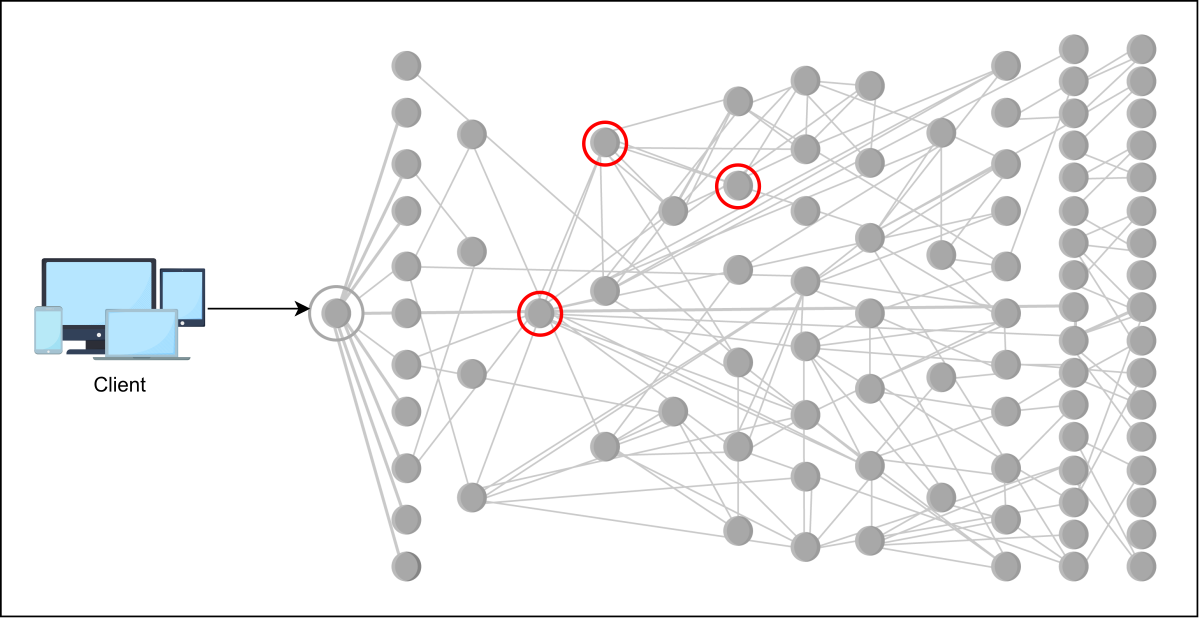
\includegraphics[width=\textwidth]{Images/chapter_22/section_5621964999229440/5752404919058432.png}
 \caption{Another service that was dependent on the previous service also failed because of it}
 \end{subfigure}
\end{figure}

\begin{figure}[htbp]
 \centering
 \begin{subfigure}[b]{0.48\textwidth}
 \centering
 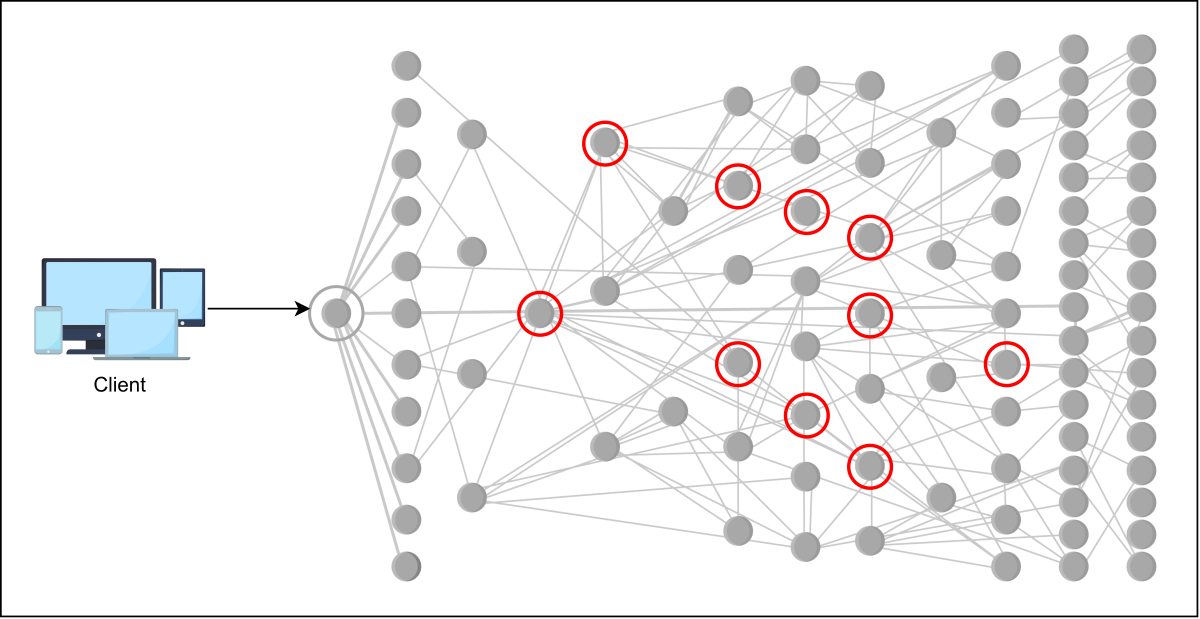
\includegraphics[width=\textwidth]{Images/chapter_22/section_5621964999229440/4698676233371648.png}
 \caption{Similarly, other dependent services also fail}
 \end{subfigure}
 \hfill
 \begin{subfigure}[b]{0.48\textwidth}
 \centering
 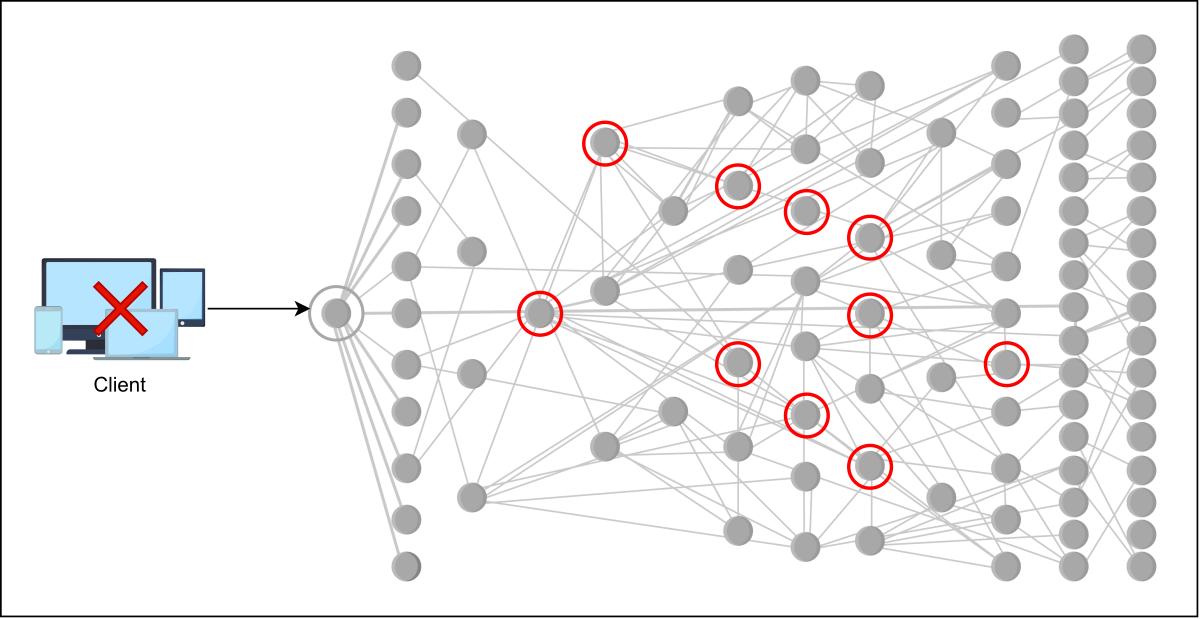
\includegraphics[width=\textwidth]{Images/chapter_22/section_5621964999229440/4630986374381568.png}
 \caption{The chain of failures in distributed systems leaves the client in an uncertain/failed state}
 \end{subfigure}
\end{figure}

\begin{figure}[htbp]
 \centering
 \begin{subfigure}[b]{0.48\textwidth}
 \centering
 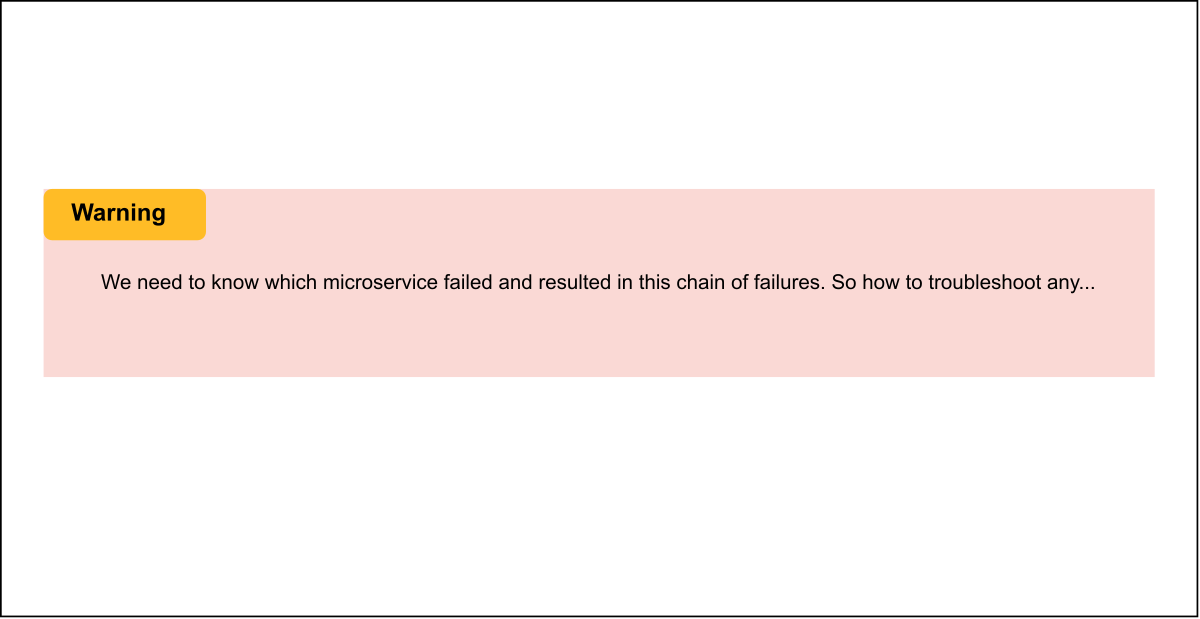
\includegraphics[width=\textwidth]{Images/chapter_22/section_5621964999229440/4738394681638912.png}
 \caption{Warning!}
 \end{subfigure}
\end{figure}

\subsection{Restrain the log size}\label{Restrain-the-log-size}
\\
The number of logs increases over time. At a time, perhaps hundreds of concurrent messages need to be logged. But the question is, are they all important enough to be logged? To solve this, logs have to be structured. We need to decide what to log into the system on the application or logging level.

\subsubsection{Use sampling}\label{Use-sampling}
\\
We'll determine which messages we should log into the system in this approach. Consider a situation where we have lots of messages from the same set of events. For example, there are people commenting on a post, where Person X commented on Person Y's post, then Person Z commented on Person Y's post, and so on. Instead of logging all the information, we can use a~\textbf{sampler service}~that only logs a smaller set of messages from a larger chunk. This way, we can decide on the most important messages to be logged.
\begin{quote}
\textbf{Note:}~For large systems like Facebook, where billions of events happen per second, it is not viable to log them all. An appropriate sampling threshold and strategy are necessary to selectively pick a representative data set.
\end{quote}
\\
We can also categorize the types of messages and apply a filter that identifies the important messages and only logs them to the system.

\begin{quote}
\textbf{Quiz:}
\textbf{Question 1:} What is a scenario where the sampling approach will not work?
\textbf{Answer:} Let's consider an application that processes a financial ATM

transaction. It runs various services like fraud detection, expiration time checking, card validation, and many more. If we start to miss out logging of any service, we cannot identify an end-to-end flow that affects the debugging in case an error occurs. Using sampling, in this case, is not ideal and results in the loss of useful data.
\end{quote}

\subsubsection{Use categorization}\label{BIvSsrNVDZK5_JtO68EdH}
\\
Let's look into the logging support provided by various programming languages. For example, there's log4j and logging in Python. The following severity levels are commonly used in logging:

\begin{itemize}
\item
\protect\phantomsection\label{u1XnMrVa322aRXs-XJkKp}
\texttt{DEBUG}
\item
\protect\phantomsection\label{NKGPghi5qXy9WH96KEj52}
\texttt{INFO}
\item
\protect\phantomsection\label{1fEBlka44_NDBTrutKJqI}
\texttt{WARNING}
\item
\protect\phantomsection\label{hurVv1ovn0si6zQF7jJtJ}
\texttt{ERROR}
\item
\protect\phantomsection\label{lf5atEbPm1FWDr4_r2N57}
\texttt{FATAL/CRITICAL}
\end{itemize}
\\
Usually, the production logs are set to print messages with the severity of \texttt{WARNING} and above. But for more detailed flow, the severity levels can be set to \texttt{DEBUG} and \texttt{INFO} levels too.
\\
Click on the ``Run'' button to see the execution of an example that uses Python's logging library to print logs.

\begin{lstlisting}[language=Python]
import logging as log
# set the logging level to DEBUG
log.basicConfig(level=log.DEBUG)
for i in range(6):
    if i == 0:
        log.debug("Debug level")
    elif i == 1:
        log.info("Info level")
    elif i == 2:
        log.warning("Warning level")
    elif i == 3:
        log.error("Error level")
    elif i == 4:
        log.critical("Critical level")
    elif i == 5:
        print("Uncomment the following to view a system generated error:")
        #print(3/0)
\end{lstlisting}

\begin{quote}
The output will be similar to:

\begin{verbatim}
DEBUG:root:Debug level
INFO:root:Info level
WARNING:root:Warning level
ERROR:root:Error level
CRITICAL:root:Critical level
\end{verbatim}
\end{quote}
\\
Let's uncomment \textbf{line 17} to view a system-generated error over the division of an integer by zero. Python itself logs the error to the console:

\subsection{Structure the logs}\label{W3ApynimIMVPan1jXATs8}
\\
Applications have the liberty to choose the structure of their log data. For example, an application is free to write to log as binary or text data, but it is often helpful to enforce some structure on the logs. The first benefit of structured logs is better interoperability between log writers and readers. Second , the structure can make the job of a log processing system easier.
\begin{quote}
\textbf{Note:} The structuring of logs is a dense topic in itself. We refer the interested learners to the PhD thesis by Ryan Braud titled "Query-based debugging of distributed systems "
\end{quote}
\subsection{Points to consider while logging}\label{y1jGXw_ybPk1RopvQzC2_}
\\
We should be careful while logging. The logging information should only contain the relevant information and not breach security concerns. For secure data, we should log encrypted data. We should consider the following few points while logging:

\begin{itemize}
\item
\protect\phantomsection\label{CuxvZuc9CVnMhTO7nDCML}
Avoid logging personally identifiable information (PII), such as names, addresses, emails, and so on.
\item
\protect\phantomsection\label{E_bhC60O8TYdFc_SuFQWE}
Avoid logging sensitive information like credit card numbers, passwords, and so on.
\item
\protect\phantomsection\label{hRVf7ym_BR9iGhJvS7vlJ}
Avoid excessive information. Logging all information is unnecessary. It only takes up more space and affects performance. Logging, being an I/O-heavy operation, has its performance penalties.
\item
\protect\phantomsection\label{tryS21oXUdfExOW9BfycZ}
The logging mechanism should be secure and not vulnerable because logs contain the application's flow, and an insecure logging mechanism is vulnerable to hackers.
\end{itemize}
\\
What are the challenges in using traditional logging in a distributed system?\\
\\
Use the AI assessment widget below to submit your solution and get an interactive response.

\textbf{Question:}

What are the challenges in using traditional logging in a distributed system?

\textbf{Reference Answer:}

The main challenges include:

\begin{itemize}
\tightlist
\item
Difficulty in tracing logs across multiple services and nodes.\\
\item
Huge volume of logs generated, making it hard to manage.\\
\item
Ensuring security and privacy of sensitive data in logs.\\
\item
Ensuring logs are available and searchable across globally distributed systems.
\end{itemize}

\subsubsection{Vulnerability in logging infrastructure}\label{HTa1rm1U31BsQdAoiQuRY}
\\
A \textbf{zero-day vulnerability} in Log4j, a famous logging framework for Java, has been identified as of November 2021. Log4j has contained the hidden vulnerability, Log4Shell (CVE-2021-44228), since 2013. Apache gave the highest available score, a CVSS severity rating of 10, to Log4Shell. The exploit is simple to execute and affects hundreds of millions of devices. Security experts are convinced that this vulnerability can allow devastating cyberattacks internationally because it can enable attackers to run malicious code and take control of the machine.

% End of section content